\documentclass[12pt]{article}

\usepackage{fixltx2e}
\usepackage{textcomp}
\usepackage{fullpage}
\usepackage{amsfonts}
\usepackage{verbatim}
\usepackage[english]{babel}
\usepackage{pifont}
\usepackage{color}
\usepackage{setspace}
\usepackage{lscape}
\usepackage{indentfirst}
\usepackage[normalem]{ulem}
\usepackage{booktabs}
% \usepackage{nag}
\usepackage{natbib}
% \usepackage{bibtex}
\usepackage{float}
\usepackage{latexsym}
\usepackage{hyperref}
\usepackage{url}
% \usepackage{html}
\usepackage{epsfig}
\usepackage{graphicx}
\usepackage{amssymb}
\usepackage{amsmath}
\usepackage{bm}
\usepackage{array}
%\usepackage{mhchem}
\usepackage{ifthen}
\usepackage{caption}
\usepackage{xcolor}
\usepackage{amsthm}
\usepackage{amstext}
\usepackage{nicefrac}
\usepackage{algorithm}
\usepackage{algorithmic}
\usepackage[scientific-notation=true]{siunitx}
\usepackage{subfigure}
\usepackage[flushleft]{threeparttable}
\usepackage{lineno}
\usepackage{adjustbox}
\usepackage{ragged2e}
\usepackage{authblk}
\usepackage{multirow}
\usepackage[T1]{fontenc}

\setlength{\parskip}{1em}
\renewcommand{\baselinestretch}{2.0}
\renewcommand\Affilfont{\small}

\begin{document}

\title{StarBEAST2 brings faster species tree inference and accurate estimates of substitution rates}
\author[1,2]{Huw A. Ogilvie\thanks{huw.ogilvie@anu.edu.au}}
\author[2,3]{Alexei J. Drummond}
\affil[1]{Division of Evolution, Ecology and Genetics, Research School of Biology, Australian National University, Canberra, Australia}
\affil[2]{Centre for Computational Evolution, University of Auckland, Auckland, New Zealand}
\affil[3]{Department of Computer Science, University of Auckland, Auckland, New Zealand}

\maketitle

\clearpage

\justifying

\section*{Abstract}

The multispecies coalescent (MSC) reconstructs species trees from a set of
genes, and fully Bayesian MSC methods like *BEAST estimate species trees from
multiple sequence alignments. Today thousands of genes can be sequenced for a
given study, but using that many genes with *BEAST is intractably slow. One
alternative is concatenation, which assumes that the evolutionary history of
each gene tree is identical to the species tree. This is an inconsistent
estimator of species tree topology, and a worse estimator of divergence times.
Concatenation also induces spurious substitution rate variation when incomplete
lineage sorting is present. Another alternative is to use summary MSC methods
like ASTRAL, but such methods are also unsatisfactory because they infer branch
lengths in coalescent units, and so cannot estimate divergence times. To enable
fuller use of available data and more accurate inference of species tree
topologies, divergence times, and substitution rates, we have developed a new
version of *BEAST called StarBEAST2. To improve convergence rates we add
analytical integration of population sizes and novel MCMC operators which
improved computational performance by 3.1$\times$ when analyzing a single
empirical data set, and an average of 6.2$\times$ across 96 simulated data sets.
Convergence rates are also more consistent between chains than *BEAST. To enable
accurate estimates of per-species substitution rates we introduce species tree
relaxed clocks, and show that StarBEAST2 is a more powerful and robust estimator
of rate variation than concatenation. StarBEAST2 is available through the BEAUTi
package manager in BEAST 2.4 and above.

Keywords: Multispecies coalescent, concatenation, phylogenetic methods, incomplete lineage sorting, relaxed clocks, species trees.

\section{Introduction}

The throughput of sequencing technologies has improved many-fold over the past
two decades culminating in next generation sequencing (NGS), and it is now
feasible to sequence whole or partial genomes or transcriptomes for phylogenetic
studies \citep{annurev-ecolsys-110512-135822}. NGS produces hundreds or
thousands of phylogenetically useful loci \citep[see for example][]{Blom20160181}
with potentially millions of sites spread across a data set of multiple
sequence alignments.

While NGS offers hundreds or thousands of loci at relatively low cost, making
accurate inferences from the enormous amount of data produced is particularly
challenging. In the case of *BEAST, a fully Bayesian method of species tree
inference which implements a realistic and robust evolutionary model in the
multispecies coalescent \citep[MSC;][]{Degnan2009332, Heled01032010}, it becomes exponentially
slower as the number of loci in an analysis is increased. This scaling behaviour
causes *BEAST to become intractably slow after a certain number of loci
\citep[the exact number will depend on other parameters of the data set, see][]{Ogilvie01052016}.
Given the current challenges of using large phylogenomic data sets with *BEAST
there have been three broad alternatives available to researchers; concatenate
sequences from multiple loci, use alternative MSC methods which are based on
summary statistics instead of sequence alignments, or choose a tractable
subset of loci to use with a fully Bayesian method like *BEAST, BEST \citep{Liu01112008}, or BPP
\citep{Yang854}.

Using maximum likelihood phylogenetic methods to infer a species tree based on concatenated
sequences will return the single tree that
best fits the combined sequence alignment according to the phylogenetic likelihood function \citep{Felsenstein1981}. Popular maximum-likelihood concatenation methods include
RAxML, PAML and PhyML \citep{Stamatakis01052014,
Yang01082007,Guindon01052010}. Bayesian methods, such as ExaBayes and BEAST
\citep{Aberer01102014, Drummond2007}, will instead return a distribution of trees which are probable
given the combined sequence alignment, a set of priors, and the same likelihood function.
Recent results show that likelihood-based concatenation
can be counterproductive, producing statistically inconsistent results which assign
high confidence to incorrect nodes due to model misspecification
\citep{NYAS:NYAS12747}. In the so-called ``anomaly zone'' of short branch
lengths, the most probable gene tree topology will be different from the species
tree, and estimated tree topologies will likely differ from the true species
tree topologies \citep{journal.pgen.0020068, Kubatko01022007}.

More recently identified problems with likelihood-based concatenation are systematic errors when
estimating branch lengths, including overestimation of divergence times. Because
some time is required for genes to coalescence looking backwards from
a speciation event, the expected molecular distance between two species is
greater than the true divergence time. This leads concatenation to overestimate
the divergence times across a species tree in proportion to effective population size
\citep{doi:10.1146/annurev.ecolsys.33.010802.150500}. Such overestimation of divergence times can result in dramatic
inflation of estimated tip branch lengths \citep{Ogilvie01052016}.

Incomplete lineage sorting (ILS) also causes systematic errors in estimated
branch lengths when using concatenation, because substitutions on a discordant gene tree branch
which has no corresponding species tree branch must be explained by multiple
substitutions on different species tree branches. Substitutions
produced by ILS (SPILS) causes concatenation to overestimate the lengths of specific
branches and underestimate the lengths of others, which produces apparent
substitution rate variation where none exists \citep{Mendes01072016}. For all
the above reasons, trees
inferred using concatenation are therefore not a reliable approximation of the
species tree in terms of branch lengths or topology.

As an alternative to concatenation, MSC methods which use summary statistics instead
of sequence alignments have been developed for use with phylogenomic data.
Popular summary methods include MP-EST and ASTRAL \citep{Liu2010,
Mirarab01092014}, but recent results show that MP-EST should be used with caution as it is
sensitive to gene tree errors \citep{Mirarab15062015, Xi201563}. At low levels of
ILS, MP-EST is less accurate than likelihood-based or neighbor-joining concatenation at
inferring topologies, and even at high levels of ILS it may be no more accurate
than concatenation \citep{Ogilvie01052016}. While other summary methods like
ASTRAL may be more reliable than MP-EST, these methods estimate branch lengths
in coalescent units instead of substitutions. Molecular-clock informed divergence times therefore cannot be
reconstructed using summary methods. If concatenation is used to estimate branch
lengths or divergence times for a fixed species tree
topology estimated using a summary method, then those estimates will be
unreliable for the same reasons as pure concatenation.

With the aim of improving the computational performance of fully Bayesian
MSC inference of species trees, we have developed an upgrade
to *BEAST --- StarBEAST2 --- which is available as a package for BEAST 2
\citep{10.1371/journal.pcbi.1003537}. By improving computational performance,
StarBEAST2 should enable the use of more loci and thereby improve the precision
of estimated parameters and provide an alternative to concatenation. We have
also developed and include in StarBEAST2 new MSC relaxed
clock models to enable accurate inference of per-species substitution rates.

\section{New Approaches}

\subsection{Analytical integration of population sizes}

Markov Chain Monte Carlo (MCMC) methods like *BEAST jointly integrate
over many parameters by proposing small changes at each step to eventually
produce a probability distribution for all parameters. From a
researcher's perspective, some may be ``nuisance'' parameters not of scientific
interest. For example species tree topology and divergence times may be of
interest, but not effective population sizes. For tractable parameters, an
analytic solution will integrate over the entire range of values at each MCMC
step, and may be faster than MCMC integration. However explicit
estimates will not be produced so this approach is suitable only for nuisance
parameters. Among-site rate variation is already integrated out at each step;
the likelihood of each site is calculated for all possible discrete gamma rates
at each step, so individual site rates are not estimated \citep{Yang1994}.

Analytical integration of constant per-branch population sizes was first
implemented as part of BEST \citep{EVO:EVO414}. The analytic solution, which we
have added to StarBEAST2, uses an inverse gamma conjugate prior for population
sizes. By default StarBEAST2 fixes the shape of the distribution $\alpha = 3$
and only estimates the mean of the distribution $\mu$, which is proportional to the
scale parameter $\beta$:

\begin{equation}
\mu = \frac{\beta}{\alpha - 1} = \frac{\beta}{2}
\end{equation}

In this special case where $\alpha = 3$, the standard deviation is identical to
the mean:

\begin{equation}
\sigma = \sqrt{\frac{\beta^2}{(\alpha - 1)^2 \times (\alpha - 2)}} = \sqrt{\frac{\beta^2}{2^2}} = \frac{\beta}{2} = \mu
\end{equation}

The coefficient of variation $c_\mathrm{v} = \nicefrac{\sigma}{\mu}$ of the
prior distribution for effective population sizes is therefore 1.

\subsection{Coordinated tree topology changing operators}

One approach to improving the performance of MSC analyses which simultaneously
estimate gene and species trees (such as *BEAST) is to develop MCMC operators
which propose coordinated changes to both the species tree and the gene trees in
the same step. \cite{Yang01122014} introduced a Metropolis-Hastings \citep[MH;][]{Metropolis1953, Hastings1970}
operator which makes nearest-neighbor interchange (NNI) changes to the species
tree topology, and simultaneously makes changes to gene tree topologies which
preserve compatibility of the gene trees within the proposed species tree.
Later, both \cite{Jones2016} and \cite{2015arXiv151203843R} introduced more
general coordinated operators which make subtree prune and regraft (SPR) changes
to the species tree. We have reimplemented these coordinated NNI and SPR moves
in StarBEAST2 as a single new operator called ``CoordinatedExchange''.
\cite{2015arXiv151203843R} also describe a proposal distribution which favours
topological changes on shorter branches, and also less radical changes in
topology. StarBEAST2 implements a simpler proposal distribution but still
favours less radical changes by applying adjustable proposal probability weights
to (less radical) NNI moves and (more radical) SPR moves.

\subsection{Coordinated node height changing operators}

A novel class of coordinated Metropolis operators was introduced by
\cite{Jones2016}. These operators change the height of a non-root non-leaf
species tree node, and the heights of ``connected components'' of gene tree
nodes, by an amount $\epsilon$ chosen from a uniform distribution.
The lower bound of the uniform distribution is the negative length of
the shortest child branch of any connected component or of the species tree node,
and the upper bound is the positive length of the shortest parent branch. As
long as the connected components are chosen with reference only to the topology
of the species tree, the topology of the gene trees, and the mapping of
sampled individuals to species, operators of this class are symmetric
\citep{Jones2016}.

We have developed a new operator called ``CoordinatedUniform'' that belongs to
this class. Individuals from extant species which descend from a species tree
node, or are directly descended from a gene tree node, are referred to as
descendant individuals. The gene tree nodes selected by this operator to be shifted in height are those
for which (1) at least one descendant individual is also a descendant individual
of the left child of the selected species tree node, (2) the same but for the right child, and (3) all descendent
individuals are also descendent individuals of the selected species tree node.

We have also developed a new adaptive MH \citep{Andrieu2008} operator called
``CoordinatedExponential'' which changes the height of the species tree root and
the height of connected components of gene tree nodes by an amount $\epsilon$.
Just as for CoordinatedUniform, the changed gene tree nodes are those for which at least one descendant individual
is also a descendant individual for each child of the species tree root.
Because the length of parent branches of the species tree root or connected
components which include a gene tree root will be undefined, a different method must be used to choose
$\epsilon$ compared to CoordinatedUniform.

First the lower bound of the species tree root height is defined as the current
height minus the length of the shortest child branch of any connected component or
of the species tree root. The difference between the lower bound and the current
root height is referred to as $x$, and a new random value $x'$ is chosen from an
exponential distribution. The value of $x' - x$ is then used for $\epsilon$. The
median of the exponential distribution is adaptively modified over the course of
an MCMC chain to equal the posterior expectation of $x$.

Because the proposal distribution for a new species tree root height is
independent of the current height, the Hastings ratio which is usually
$\nicefrac{q(x',x)}{q(x,x')}$ \citep{Hastings1970} can be simplified to
$\nicefrac{\pi(x)}{\pi(x')}$. The natural logarithm of the Hastings ratio may then
be derived from the respective probability densities of $x$ and
$x'$ drawn from an exponential distribution with the rate $\lambda$:

\begin{align}
\frac{\pi(x)}{\pi(x')} &= \frac{\lambda e^{-\lambda x}}{\lambda e^{-\lambda x'}} = \frac{e^{-\lambda x}}{e^{-\lambda x'}}\\
\therefore \ln\left(\frac{\pi(x)}{\pi(x')}\right) &= \ln \left(e^{-\lambda x}\right) - \ln \left(e^{-\lambda x'}\right)\\
& = \lambda x' \cdot \ln \left(e\right) - \lambda x \cdot \ln \left(e\right)\\
& = \lambda \left(x' - x\right) = \lambda \epsilon
\end{align}

\subsection{Species tree relaxed clocks}

The overall rate of evolution occurring at a given locus within a species will
be influenced by the nature of the particular gene and also by the natural
history of the particular species. For a given gene, the average substitution
rate may depend on the effects of selection such as the accelerated molecular
evolution of sex-biased genes in \textit{Arabidopsis thaliana}
\citep{Gossmann01032014}, or on within-genome variation in mutation rate \citep{Baer2007}.
For a given species, the average substitution rate is correlated with a
multitude of traits including metabolic rate, body size, and fecundity, although
causal relationships are difficult to pin down \citep{Bromham2503}.
Unsurprisingly in light of the above, empirical analysis has shown that two
major factors contributing to rate variation among gene branches are the
per-gene rate and the per-species rate \citep{Rasmussen01122007}.

Because variation is expected in the nature of different genes and species, and
therefore variation is also expected in the average substitution rate of different
genes and species, multispecies coalescent models should take both per-gene and
per-species rate variation into account. *BEAST can accommodate both types of
rate variation using gene tree relaxed clock models \citep[for examples see][]{Berv2014120, Lambert2015146}.
This involves estimating per-branch substitution rates separately
for each branch of each gene tree. While gene tree relaxed clocks may
accommodate variation in substitution rates between species, they do not produce
estimates of species branch rates. To enable accurate inference of species
branch rates, we have developed a new species tree relaxed clock model.

The challenge of applying a relaxed clock to the species tree is that
phylogenetic likelihood calculations require branch rates for each branch of
each gene tree. Our clock model computes those rates using the total expected number of substitutions
$\Sigma \mathbb{E}(S)$ accumulated by a gene branch through all containing
species branches. Substitutions are expected to be accumulated at the mean
clock rate of the gene tree $c$, for example 0.01 for hominoid primate
mitochondrial DNA \citep{doi:10.1146/annurev.es.18.110187.001413}, multiplied
by the lengths of time $L$ spent traversing each species tree branch, multiplied
by the rates $R$ of the corresponding species tree branches
(Table~\ref{tab:branchRateModel}).

\begin{table*}[htb!]
\caption{Expected numbers of substitutions $\Sigma \mathbb{E}(S)$ under a species tree relaxed clock}
\label{tab:branchRateModel}
\begin{threeparttable}
\begin{tabular*}{\textwidth}{@{\extracolsep{\fill}}cccccccccccc@{}}
\hline
Gene & Gene & \multicolumn{3}{c}{Length within $L$} & \multicolumn{3}{c}{Species rate $R$} & \multicolumn{3}{c}{$\mathbb{E}(S) = c\cdot L\cdot R$} & \multirow{2}{*}{$\Sigma \mathbb{E}(S)$}\tabularnewline
branch & rate $c$ & A & B & AB & A & B & AB & A & B & AB & \tabularnewline
\hline
a & \multirow{2}{*}{0.01} & 1.0 & 0.0 & 0.5 & \multirow{2}{*}{0.7} & \multirow{2}{*}{1.0} & \multirow{2}{*}{1.3} & 0.0070 & 0.0000 & 0.0065 & 0.0135\tabularnewline
b & & 0.0 & 1.0 & 0.5 & & & & 0.0000 & 0.0100 & 0.0065 & 0.0165\tabularnewline
\hline
\end{tabular*}
\end{threeparttable}
\end{table*}

The gene tree branch rates $r$ can then be derived by dividing the total
expected number of substitutions by the total length of that branch $l$. The
gene tree branch rates for the illustrated example
(Figure~\ref{fig:branchRateModel}; Table~\ref{tab:branchRateModel}) are
therefore:

\begin{align}
r_a &= \frac{\Sigma \mathbb{E}(S_a)}{l_a} = \frac{0.0135}{1.5} = 0.009\\
r_b &= \frac{\Sigma \mathbb{E}(S_b)}{l_b} = \frac{0.0165}{1.5} = 0.011
\end{align}

The new species tree relaxed clock model is available in StarBEAST2. Branch rate
models that can be used with a species tree relaxed clock currently include the
well-established uncorrelated log-normal (UCLN) and uncorrelated exponential
(UCED) models \citep{10.1371/journal.pbio.0040088}, as well as the newer random
local clock model \citep{Drummond2010}.

\begin{figure}[htb!]
\centering
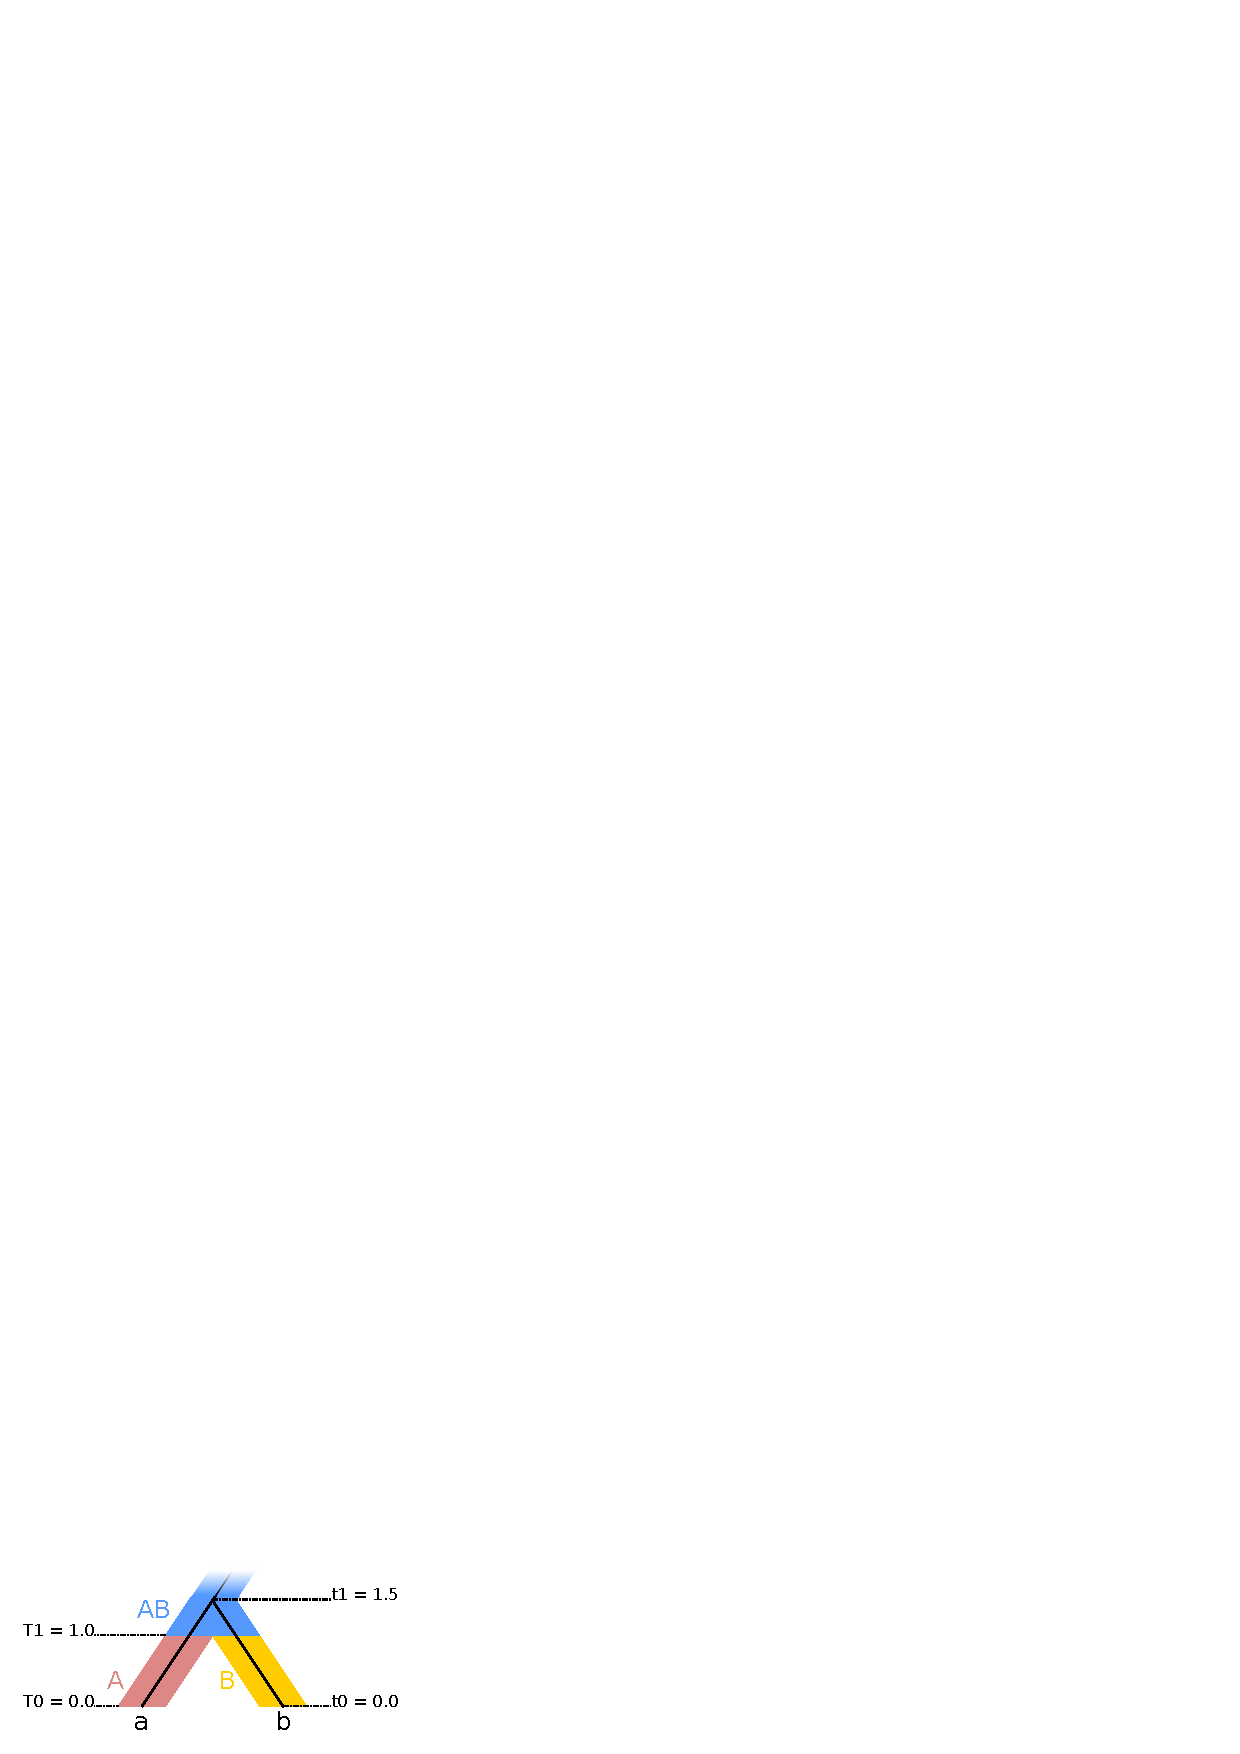
\includegraphics[width=2.5in]{relaxed_clock.pdf}
\caption
{Two-species phylogeny used to illustrate species tree relaxed
clocks. There are two extant species ``A'' and ``B'', and one ancestral species ``AB''.
Within the species tree there is a single gene tree with extant individuals ``a''
and ``b''. The single speciation event occurs at time T1, and the single coalescence
event occurs at time t1.}
\label{fig:branchRateModel}
\end{figure}

\section{Results}

\subsection{StarBEAST2 correctly implements the multispecies coalescent}

New methods must be shown to be correct implementations of the
target model. One way to accomplish this for MCMC methods is to estimate
parameters from a prior distribution using the MCMC kernel, and to also draw
independent samples from the same distribution by simulation. The resulting
parameter distributions should be identical if the implementation is correct. We
used this method to test the correctness of the novel features in StarBEAST2;
analytical population size integration, coordinated operators, and species tree
relaxed clocks. Simulated and StarBEAST2 distributions were identical
for species and gene tree topologies (Figure~S1,S2), species and gene tree node
heights (Figure~S3,S4), and for gene tree branch rates (Figure~S5,S6). This
combination of results supports the correctness of the StarBEAST2
implementation.

\subsection{\textit{Pseudacris} chorus frogs have intermediate coalescent branch lengths}

To characterize the performance of coordinated operators, methods of population size
integration and relaxed clocks, we tested StarBEAST2 using real sequence data.
The data set used for this analysis is from the North American chorus frog genus
\textit{Pseudacris}, and was originally collected and analyzed by
\cite{Barrow201478}. A key metric of phylogenies that can be used to judge
whether it is necessary to employ MSC models is the average
branch length in coalescent units $\nicefrac{\tau}{2N_e}$. Given short branch
lengths, likelihood-based or neighbor-joining concatenation is unable to infer accurate species trees regardless of
the number of loci used, but for long branch lengths, concatenation is
approximately as accurate as *BEAST \citep{Ogilvie01052016}. Using StarBEAST2,
the average branch length within this genus was determined to be
$\nicefrac{3.22\tau}{2N_e}$. This is an intermediate average length compared to
the shallow simulations analyzed by \cite{Ogilvie01052016} which had a shorter
average length of $\nicefrac{0.54\tau}{2N_e}$.

\subsection{Coordinated height changing operators and analytical integration improve performance}

To determine which configuration of new features would achieve the best
performance, we ran StarBEAST2 using different combinations of operators,
methods of population size integration and different relaxed clocks. To measure
convergence both effective sample size (ESS) per hour and ESS per million states
were computed for each independent chain. ESS per hour can be used to calculate
the total time required for a converged chain (nominally where ESS equals or
exceeds 200), and reflects how effectively operators explore the space of trees
and parameters, as well as the computational time required by each operator
proposal and likelihood calculation. In contrast, ESS per million states
reflects only the exploration of tree and parameter space independently of
calculation times. A variety of statistics were recorded for each analysis
(Table~S1-S4), and for each replicate the statistic with the slowest ESS rate
for that particular chain was used when computing the mean and standard
deviation of ESS per hour and per million states.

Multiple linear regressions with log transformed ESS rates as the response
variables were used to measure the effect of coordinated topology changing operators,
coordinated node height changing operators, and the method of population size
integration. Each additional feature was treated as a binary indicator variable
so that we could quantify the relative performance as a percentage by
exponentiating the coefficient for each addition
(Table~\ref{tab:convergenceLM}). An interaction term for height changing
operators and population size integration was included because visualization of
ESS rates (Figure~\ref{fig:realEssPerHour}) suggested such an interaction existed.

\begin{table*}[htb!]
\caption{Relative performance of operators, population size integration and clock models applied to \textit{Pseudacris} reanalyses.}
\label{tab:convergenceLM}
\begin{threeparttable}
\begin{tabular*}{\textwidth}{@{\extracolsep{\fill}}rlrrrr@{}}
\hline
Relaxed clock & ESS rate per & Topology & H(eight) & A(nalytical) & H $\times$ A\tabularnewline
\hline
Gene trees & hour & 83\%{***} & 247\%{***} & 107\%\hphantom{***} & 131\%{**}\hphantom{*}\tabularnewline
Gene trees & million states & 101\%\hphantom{***} & 278\%{***} & 110\%\hphantom{***} & 130\%{*}\hphantom{**}\tabularnewline
Species tree & hour & 91\%\hphantom{***} & 753\%{***} & 110\%\hphantom{***} & 124\%{*}\hphantom{**}\tabularnewline
Species tree & million states & 106\%\hphantom{***} & 805\%{***} & 113\%\hphantom{***} & 124\%{*}\hphantom{**}\tabularnewline
\hline
\end{tabular*}
\begin{tablenotes}
\item {*}: $p < 0.05$, {**}: $p < 0.01$, {***}: $p < 0.001$.
\end{tablenotes}
\end{threeparttable}
\end{table*}

Coordinated topology operators had a significantly negative effect on ESS per
hour of gene tree relaxed clock analyses, but no significant effect on ESS per
million states (Table~\ref{tab:convergenceLM}), suggesting that coordinated
topology operators are no more effective than na\"ive operators at proposing new
states. A decrease in the number of states per hour (Figure~S8) shows that they
are more computationally expensive than na\"ive operators, and explains the
negative effect on ESS per hour.

\begin{figure*}[htb!]
\centering
\includegraphics[width=\textwidth]{minimum_ess_per_hour_boxplot.pdf}
\caption
{Impact of operators, population size integration and clock models on
convergence of \textit{Pseudacris} reanalyses. The estimated sample size (ESS)
per hour for a given replicate used the smallest ESS out of all recorded
statistics. Topology refers to the replacement of na\"ive nearest-neighbor
interchange and subtree prune and regraft operators with coordinated operators.
Height refers to the addition of operators which make coordinated changes to
node heights. Uncorrelated log-normal (UCLN) relaxed clocks were applied to
either each gene tree or to the species tree. N = 32.}
\label{fig:realEssPerHour}
\end{figure*}

For gene tree and species tree relaxed clock analyses, convergence rates
using coordinated height changing operators were 2.47 times and 7.53 times
as fast respectively than
without those operators (Table~\ref{tab:convergenceLM}). The
difference made to species tree relaxed clock performance
suggests that coordinated height changing operators are necessary for practical
implementations of that model (Figure~\ref{fig:realEssPerHour}).

Species tree relaxed clocks with coordinated height changing operators were
faster in terms of ESS per million states than gene tree relaxed clocks
(Figure~S7), showing that new state proposals are more effective. However
changing a species tree branch rate requires updating the phylogenetic
likelihood for all gene trees so the computational cost is much higher than for
gene tree relaxed clocks (Figure~S8), so species tree relaxed clocks are still
moderately slower than gene tree relaxed clocks in terms of ESS per hour
(Figure~\ref{fig:realEssPerHour}).

In the absence of coordinated height changing operators, analytical population
size integration had no significant effect on performance under any
circumstance. However when combined with those operators, significant increases
to ESS per hour and ESS per million states were observed for both gene tree and
species tree relaxed clock analyses (Table~\ref{tab:convergenceLM}).

\subsection{Species tree relaxed clocks prevent SPILS}

When using concatenation to infer a species tree, SPILS causes apparent
substitution rate variation among predictable species tree branches. However in
an ultrametric (time tree) framework like BEAST, branch lengths are constrained so that
terminal species begin at time zero. We hypothesized that if a relaxed clock is
used with concatenation in an ultrametric framework, SPILS will be absorbed as
faster substitution rates for lineages that would be lengthened by SPILS in a
non-ultrametric framework.

In an ultrametric framework with a strict clock and no external (e.g. fossil,
biogeographical or known clock rate)
calibrations, the substitution rate of each branch is set to 1. This ensures that 1 unit of time
is equivalent to 1 expected substitution. Using a relaxed clock with no external calibrations
the substitution rate of each branch can vary, but the expectation of the mean rate of all
branches is 1, preserving the relationship of 1 unit of time = 1 expected substitution.
Therefore when SPILS causes the rates of some branches to be faster than 1,
the rates of other branches will be slower than 1 to keep the expected mean constant.

We used BEAST concatenation and StarBEAST2 with a species tree relaxed clock to
infer the branch lengths and substitution rates of simulated species trees with
the topology ((((A,B),C),D),E), using sequence alignments simulated using a strict
clock. Gene tree discordance will increase the estimated length of A, B and C
branches for these species trees \citep{Mendes01072016}, and as hypothesized
substitution rates for A and B branches inferred using concatenation were biased
towards being faster than the true rate of 1 (Figure~\ref{fig:spilsRates}).
Estimated substitution rates for the C branch were more variable, and could be
faster or slower than 1. Substitution rates estimated for the D and E branches
were biased towards being slower than 1, presumably to balance the mean rate. Concatenation also overestimated the lengths of tip branches, another known
bias when using concatenation to infer a species tree \citep{Ogilvie01052016}. No biases were observed for the branch rates or lengths estimated using StarBEAST2
(Figure~\ref{fig:spilsRates}).

\begin{figure*}[htb!]
\centering
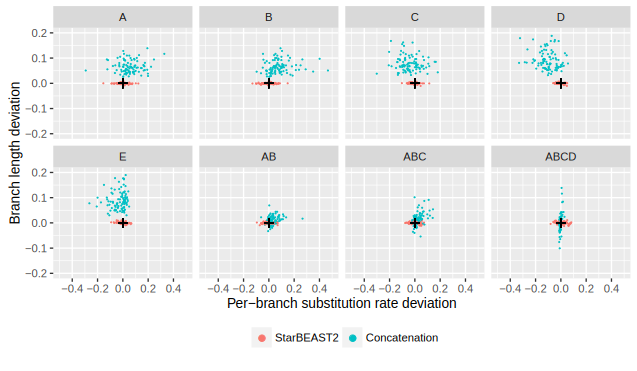
\includegraphics[width=\textwidth]{scatter.pdf}
\caption
{Accuracy of branch substitution rates and lengths inferred by BEAST
concatenation and StarBEAST2. Deviation is the difference of each estimated
rate and length from the true value. Estimated rates and lengths are the posterior
expectation of the overall substitution rate and length for each species tree
branch. Black crosses in each panel indicate the point of perfect accuracy. Each
panel shows the distributions for the labelled extant or ancestral branch. N =
96.}
\label{fig:spilsRates}
\end{figure*}

A number of estimated branch rates had 95\% credible intervals that excluded the
true rate of 1 when using concatenation. If a study is testing whether
substitution rates vary across a species tree, those branch rates could be
erroneously interpreted as faster or slower than average. In our simulations,
the clock rate of the D branch would be inferred as slower than average in 37
out of 96 replicates (Figure~S9), despite the sequence data being simulated
using a strict clock. When applying the same 95\% credible intervals to branch
lengths, the true simulated length was excluded with just two exceptions for
all tip branches across all replicates using concatenation (Figure~S10). In
contrast, no erroneous results would be inferred for branch rates given the same
data using StarBEAST2, and out of the 768 total simulated non-root branch
lengths, only five erroneous results would be inferred (Figure~S9,S10).

\subsection{StarBEAST2 is several times faster than *BEAST}

Our reanalysis of \textit{Pseudacris} sequence data shows that coordinated height changing operators,
and analytical integration of population sizes when combined with those operators,
improve convergence. To show that this increased performance is generally
applicable, and to demonstrate that StarBEAST2 can accurately reconstruct
species trees, we needed to apply StarBEAST2 to simulated data sets for
which the true species trees are known. To accomplish this we simulated 96 species
trees of 19 taxa each under a birth-death model with log-normally distributed
branch rates. Gene trees evolving within each species tree were simulated
according to the MSC model with log-normally distributed mean clock rates.
Finally, sequences were simulated according to an HKY process for each gene
\citep{Hasegawa1985, Goldman1993}. The parameters used for these simulations
were chosen to produce intermediate branch lengths in coalescent units; the
average simulated branch length was $\nicefrac{3.22\tau}{2N_e}$, the same as for
\textit{Pseudacris} to two decimal places.

Simulated data was analyzed using concatenation with BEAST and using the MSC with
StarBEAST2 with *BEAST settings,
high performance settings with gene tree relaxed clocks, and high performance settings with
species tree relaxed clocks. *BEAST settings matched the configuration of *BEAST
before StarBEAST2; explicit MCMC integration of population sizes, no
coordinated operators, na\"ive NNI and SPR topology operators, and a UCLN
relaxed clock applied to each gene tree. High performance settings included analytical
integration of population sizes, coordinated height changing operators, and
na\"ive NNI and SPR topology operators. Again multiple statistics were recorded
to compute the ESS rate means and standard deviations (Table~S5-S8).

Our simulation study confirmed that StarBEAST2 is several times faster than
*BEAST (Figure~\ref{fig:simulatedEssPerHour}). For simulated data the average
log convergence rate of StarBEAST2 with high performance settings and gene tree
relaxed clocks was 4.01 $\ln(\nicefrac{ESS}{hour})$. This compares to
2.18 using *BEAST settings, an increase in performance of
$\exp(4.01 - 2.18) = 6.2$ times (Table~S5). However
for \textit{Pseudacris} reanalyses the average was 3.66 for StarBEAST2 compared
to 2.52 for *BEAST, a smaller increase of 3.1 times (Table~S1).

Species tree relaxed clocks were slower than the gene tree relaxed clocks when
using high performance settings (Figure~\ref{fig:simulatedEssPerHour}). The
average log rate for simulated data when using a species tree relaxed clock with
high performance settings was 3.74, which is still 4.8 times faster than
using gene tree relaxed clocks with *BEAST settings (Table~S5). Again the
difference was smaller for \textit{Pseudacris} reanalyses, with a rate of 3.36
for StarBEAST2, or 2.3 times faster (Table~S1).

The computational performance of StarBEAST2 was also more consistent than
*BEAST. The standard deviations of the log rate using StarBEAST2 to analyze
simulated data sets were 0.44 and 0.46 for gene and species tree relaxed clocks
respectively, compared to 0.73 for *BEAST (Table~S7). The standard deviations
when reanalyzing \textit{Pseudacris} were 0.23, 0.26 and 0.55 for StarBEAST2
with gene tree relaxed clocks, StarBEAST2 with species tree relaxed clocks, and
*BEAST respectively. The higher spread for simulated data reflects the fact that
each replicate used a different species tree with different genes and sequence
alignments.

Concatenation with the same number of loci is much faster than StarBEAST2, but
concatenation using 220 loci was similar to *BEAST and slower than StarBEAST2
(Figure~\ref{fig:simulatedEssPerHour}).

\begin{figure}[htb!]
\centering
\includegraphics[width=2.5in]{combined_ess_per_hour.pdf}
\caption
{Convergence of different methods applied to simulated and empirical data sets. The estimated sample size (ESS) per hour for a
given replicate used the smallest ESS out of all recorded statistics. Methods are
BEAST concatenation with 22 loci, concatenation with 220 loci (10X), StarBEAST2 with
*BEAST settings and 22 loci, and StarBEAST2 with high performance settings, 22 loci,
and uncorrelated log-normal relaxed clocks applied to the gene trees (GT-UCLN) or
to the species tree (ST-UCLN). \textit{Pseudacris} results from Figure~\ref{fig:realEssPerHour} are also reproduced for
multispecies coalescent analyses (dashed-line boxes). N = 96 (simulated), N = 32
(\textit{Pseudacris}).}
\label{fig:simulatedEssPerHour}
\end{figure}

\subsection{Concatenation is a worse estimator of branch lengths than topology}

The accuracy of StarBEAST2 relative to BEAST concatenation varied depending on the
type of error and whether equal numbers of loci were used. Relative species tree
error measures the accuracy of estimated branch lengths; by that measure
StarBEAST2 using 22 loci outperformed concatenation using 22 loci, and matched
the performance of concatenation using 220 loci
(Figure~\ref{fig:speciesTreeError}A). Pendant edge bias measures systematic bias
in the estimated ages of extant species; by that measure StarBEAST2 was much
less biased even when concatenation was used with ten-fold more data
(Figure~\ref{fig:speciesTreeError}B). Rooted Robinson-Foulds distance measures
the topological accuracy of estimated trees; for that metric concatenation using
22 loci was almost as accurate as StarBEAST2, and more accurate when using
220 loci (Figure~\ref{fig:speciesTreeError}C). For no type of error did the
choice of gene or species tree relaxed clocks significantly affect the accuracy of StarBEAST2
(Figure~\ref{fig:speciesTreeError}A,B,C).

\begin{figure}[htb!]
\centering
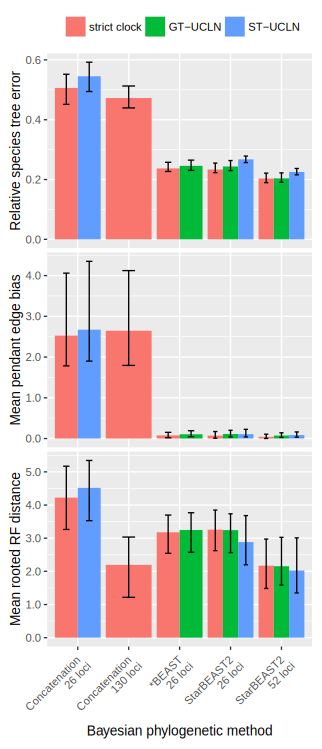
\includegraphics[width=2.5in]{tree_error.pdf}
\caption
{Accuracy of different methods applied to simulated data. Methods are BEAST concatenation with 22 loci, concatenation with 220 loci
(10X), StarBEAST2 with *BEAST settings and 22 loci, and StarBEAST2 with
high performance settings, 22 loci, and uncorrelated log-normal relaxed clocks applied
to the gene tree (GT-UCLN) or to the species tree (ST-UCLN). (A) Trimmed mean of
relative species tree error, a measure of branch length error. (B) Trimmed
mean of mean pendant edge bias, which measures biased estimates of the ages of
extant species. (C) Trimmed mean of mean rooted Robinson-Foulds (RF) distances, a
measure of topological error. 25\% trim was used to reduce the
influence of outliers. All error bars are 95\% confidence intervals calculated
by bootstrapping. N = 96.}
\label{fig:speciesTreeError}
\end{figure}

\subsection{StarBEAST2 is superior at inferring substitution rates given intermediate branch lengths}

While the convergence of species tree relaxed clock analyses was slower than for
gene tree relaxed clocks using high performance settings, species tree
relaxed clocks enable inference of species branch rates within an MSC framework.
To gauge the accuracy of estimated branch rates, we used simple linear
regressions with the true rate of each simulated branch as the explanatory
variable, and the posterior expectation of the rate of that branch (conditional
on the corresponding clade being monophyletic in the posterior samples) as the
response variable. If all estimates are equally proportional to the truth, then the $R^2$ coefficient
of determination will equal 1.

When estimating branch rates using BEAST concatenation with either 22 or 220 loci,
$R^2$ was very weak at $0.07$ and $0.09$ respectively. By applying a relaxed
clock to the species tree using StarBEAST2, the $R^2$ was much higher at $0.21$
using just 22 loci (Figure~\ref{fig:branchRates}).

The true standard deviation used to simulate branch rates was 0.16, and the
estimated standard
deviation for 220 locus BEAST concatenation analyses was 0.14. In contrast the
estimated standard deviations for 22 locus analyses were 0.08 and 0.07 for
concatenation and StarBEAST2 respectively. This is because when the sequence
alignments are less informative for a given branch (as happens when fewer loci are
used), the posterior expectation of the rate will be close to the prior
expectation which is 1. This is evident in Figure~\ref{fig:branchRates} as the
large number of branch rates around 1 for both 22 locus analyses.

\begin{figure}[htb!]
\centering
\includegraphics[width=2.5in]{branch_rates.pdf}
\caption
{Estimates of species tree branch rates using BEAST concatenation versus StarBEAST2.
Methods are concatenation with 22 loci, concatenation with 220 loci (10X), and
StarBEAST2 with high performance settings, 22 loci, and a relaxed clock applied
to the species tree. Estimated rates are the posterior expectations of each
branch rate from each replicate. Root branch rates, which were fixed at 1,
were excluded. In blue are simple linear regression lines of best fit. N = 96.}
\label{fig:branchRates}
\end{figure}

\section{Discussion}

\subsection{StarBEAST2 will enable faster and more precise inference}

The increased performance of StarBEAST2 will enable researchers to analyze
sequence data more quickly and disseminate their findings sooner; a large MCMC
analysis which would currently take six weeks might now be performed in one or two
weeks. In the case of phylogenomic data which has been subsetted for use with
*BEAST, StarBEAST2 can alternatively be used to analyze more data for more
precise estimates of species trees and other parameters in the same amount of
time as a more limited *BEAST analysis.

Our results show that convergence rate of different MCMC chains will vary
despite an identical StarBEAST2 configuration and data, as variation in ESS per
hour exists between replicate \textit{Pseudacris} runs. The
higher standard deviation for the log ESS rate of simulation replicates suggests
that additional variation comes from the particular data set being analyzed,
because each replicate used a different species tree with different genes and
sequence alignments. The \textit{Pseudacris} species tree or choice of genes to
sample may
represent a slower than average data set, as StarBEAST2 was on average 6.2 times
faster than *BEAST across the simulated data sets, compared to 3.1 times faster
for \textit{Pseudacris}.

Previous research on the scaling behaviour of *BEAST has shown that the
relationship between the number of loci in a given analysis and the convergence
in terms of ESS per hour follows a power law based on the
the number of loci with a coefficient of approximately $-2.8$ \citep{Ogilvie01052016}. If the number of loci for a
given analysis is doubled, the convergence rate is therefore
expected to be $\exp(-2.8 \cdot \ln(2)) = 0.144 \approx \nicefrac{1}{7}$ that
of the original analysis. Based on our simulation results, this suggests that
StarBEAST2 should be able to analyze datasets of approximately twice the size
that *BEAST can in the same time.

\subsection{Concatenation can still be inferior given intermediate branch lengths}

Likelihood-based or neighbor-joining concatenation cannot accurately
estimate branch lengths in substitutions when branches have short lengths in coalescent units.
*BEAST using just four loci can be more accurate than
concatenation using 4096 loci in terms of relative species tree error and
pendant edge bias. *BEAST can also be more accurate at estimating species tree
topologies given the same number of loci as concatenation, but inferior when
concatenation can be used with a much greater number of loci
\citep{Ogilvie01052016}.

We have shown that concatenation can still be inferior to *BEAST and StarBEAST2
given intermediate branch lengths. For the same number of loci, a higher
relative species tree error indicates that concatenation is less accurate at
estimating branch lengths, and a large pendant edge bias indicates that
it also tends to overestimate tip branch lengths --- equivalent to the
ages of extant species given complete species sampling. Unlike the short branch
length case, concatenation with 10 times more loci can match the multispecies
coalescent in
terms of relative species tree error, but is then slower than StarBEAST2 with
high performance settings. In other words, for intermediate branch lengths
StarBEAST2 can be just as accurate as concatenation but needs less investment in
both sequencing and computational time.

Concatenation does not perform as well as StarBEAST2 in terms of pendant edge bias
even using ten-fold as much data.
Pendant edge bias is important because many published phylogenies show evidence
of a slowdown in diversification rate \citep{Moen2014190}. If the ages of extant
species are overestimated, this will artificially reduce the number of recent
speciation events, mimicking a slowdown. We suggest that accurate inference of
changing diversification rates requires species trees inferred by fully Bayesian MSC methods
like StarBEAST2.

\subsection{The multispecies coalescent should be used to infer per-species substitution rates}

Concatenation is already known to have difficulty inferring branch lengths
because of SPILS. When a gene tree contains a branch absent from the species
tree, substitutions along that branch must be attributed to multiple species tree
branches in a concatenation analysis, lengthening those branch estimates. Conversely,
when a species tree contains a branch absent from a gene tree, no substitutions
can be attributed to that branch, which will be inferred to be shorter \citep{Mendes01072016}.
We show that by using BEAST concatenation with a relaxed
clock, the estimated substitution rate of branches lengthened by
SPILS can be increased, and estimated substitution rate of other
branches can be decreased. This causes erroneous results when asking if substitution rates
are constant across a species tree. In contrast, StarBEAST2 is resistant to
SPILS and did not produce any biased estimates.

When given intermediate branch lengths, concatenation was unable to accurately
estimate per-species substitution rates even when using 220 loci, and it is
reasonable to assume that shorter coalescent branch lengths would
exacerbate the problem. StarBEAST2 can recover many branch rates, and given a
more informative data set than our simulation study of 22$\times$400nt loci
should be able to further improve the accuracy of estimated rates to a point.
There are intrinsic limits to our ability to estimate substitution rates,
primarily that branch length is confounded with substitution rate
\citep{Thorne01092002}.

\section{Conclusions}

When estimating dates and rates, the choice is often between using a subset of
available loci with a fully Bayesian MSC method, or all available loci with
concatenation. Researchers have often opted for the second choice, but we have
shown that concatenation may not accurately estimate the ages of extant species
or per-species substitution rates, even for trees of intermediate branch lengths. The
increased performance of StarBEAST2 should further encourage the adoption of
fully Bayesian MSC methods for estimating divergence times, and the new species
tree relaxed clock will enable accurate inference of species branch rates despite
ILS. StarBEAST2 is free and open source software, and its source code and
development history is available through GitHub
(\url{https://github.com/genomescale/starbeast2}).

\section{Materials and Methods}

For all StarBEAST2 and BEAST concatenation analyses, the version of BEAST used was
2.4.1. For all simulations, the version of biopy \citep{biopy} used was 0.1.9.

\subsection{Mathematical correctness of StarBEAST2}

Simulated trees were generated using biopy, and trees sampled from a prior
distribution were generated using StarBEAST2 with all new features enabled. This
included analytical integration of population sizes, coordinated tree topology
and node height changing operators, and a species tree relaxed clock. 100,000
species trees were simulated, and 100,000 trees were sampled from the prior at a
rate of one every 1000 after a 10\% burn-in period.

Identical parameters were used for the simulation and for the StarBEAST2 run
including the prior distributions. The
number of species and haplotypes were fixed at 5 and 1 respectively.
The birth and death rates were fixed at 200 and 100 respectively. Haploid
population sizes followed an inverse gamma distribution with shape $\alpha =
3$ and scale $\beta = 0.004$. Two gene trees were sampled within each species
tree with mean clock rates of 0.5 and 2.

This procedure was repeated for both UCLN and for UCED species branch rates.
Branch rates were sampled from a lognormal or exponential distribution, in
either case with a mean of 1, discretized into 100 bins. The standard deviation
of the UCLN distribution was 0.16.

\subsection{Preprocessing of \textit{Pseudacris} sequence data}

Phased and aligned \textit{Pseudacris} sequence data was retrieved from Dryad
(\url{http://dx.doi.org/10.5061/dryad.23rc0}). In the original analysis, the HKY nucleotide substitution
model was applied to 22 out of 26 nuclear loci \citep{Barrow201478}. To simplify
our reanalysis, which was focused on performance and not reconstructing the
species tree \textit{per se}, we used only those 22 loci. To rank
individual sampled frogs by sequence quality, we counted the number of unambiguous base
calls for both haplotypes across all 22 HKY loci. To further avoid wasting
computational resources, we then reduced the sequence data to both haplotypes
from the best-sequenced individual from each of the 19 extant in-group lineages
in \cite{Barrow201478}.

\subsection{StarBEAST2 reanalysis of \textit{Pseudacris} sequence data}

For inference of \textit{Pseudacris} trees, we ran 32 independent StarBEAST2
chains for all 16 conditions for a total of 512 chains. The conditions were each
possible combination of species or gene tree relaxed clocks, analytical or
MCMC population size integration, coordinated or na\"ive topology changing
operators, and the inclusion or exclusion of coordinated height changing
operators. Each chain used the same sequence data but was an independent
estimate of convergence because a different random seed was used to initialize
each chain.

A birth-death prior was used for the species tree and both the net
diversification and extinction fraction hyperparameters were estimated. An
inverse gamma prior was used for per-branch constant population sizes with a
shape fixed at 3 and the mean population size hyperparameter was estimated.
Relative per-locus clock rates were estimated using a log-normal prior
distribution with the mean fixed at 1 in real space and the standard deviation
hyperparameter was estimated. An HKY+$\Gamma$ substitution model with four gamma
rate categories was applied to all loci and all base frequencies were estimated
separately for each locus. The HKY transition/transversion bias $\kappa$ and
gamma shape parameters were estimated and shared across all loci. The standard
deviation of the UCLN clock model was fixed at 0.16 and 0.32 for species tree
and gene tree relaxed clocks respectively, and 100 rate categories were used for
both types of relaxed clocks.

To ensure convergence of all chains, we ran each chain for an initial length of
$2^{23}$ states, sampling every $2^{10}$ states. ESS values were computed for
all recorded statistics after discarding 12.5\% of state samples as burn-in.
Recorded statistics included (1) the posterior probability, (2) the coalescent
probabilities of gene trees, (3) the overall prior probability, (4) the birth
death prior probability of the species tree, (5) the phylogenetic likelihood,
(6) the net diversification rate, (7) the extinction fraction, (8) the HKY
$\kappa$ parameter, (9) the among-site rate variation $\alpha$ parameter, (10)
the standard deviation of per-locus clock rates, (11) the mean population size,
(12) the height of the species tree, and (13) the length of the species tree.

If any recorded statistic had an ESS below 200, the chain was resumed until the
length of the chain was doubled. ESS values were then re-evaluated, again after
discarding 12.5\% of state samples. The length of the chain was continually
doubled and ESS values re-evaluated until the ESS values of all recorded
statistics were above 200. The rate at which trees and statistics were sampled
was halved with every chain doubling so that the total number of samples
remained constant.

ESS per hour was calculated by dividing the final ESS value for a given
statistic by 87.5\% of the total CPU time used by that chain to account for
burn-in. Likewise ESS per million states was calculated by dividing the final
ESS value by 87.5\% of the total number of the states in the chain, then
multiplied by one million. For all analyses of computational performance
including graphs and linear models, the ESS rate for any given chain was that of
the slowest converging statistic for that particular chain.

Average branch length in coalescent units was calculated by concatenating the
output (after discarding the first 12.5\% of states as burn-in from each chain) of all 32 chains
which used the combination of MCMC population size integration, na\"ive topology
operators, coordinated node height operators and species tree branch rates. For
every sample in the combined posterior distribution, the coalescent length of
each branch $\nicefrac{\tau}{2N_e}$ was calculated from its length in
substitution units $\tau$ and its effective population size $N_e$. The mean
coalescent length of all branches across all samples was taken as the average.

\subsection{Testing the effects of SPILS on estimated substitution rates}

To test how SPILS affected estimates of per-species branch substitution rates,
96 fully asymmetric species trees were simulated with the topology
((((A,B),C),D),E). All species trees were simulated according to a pure birth Yule
process \citep{Yule21} with a speciation rate of 10.

Haploid population sizes for each branch were chosen independently from an
inverse gamma distribution with a shape of 3 and a scale of 0.2. 100 gene trees
with one individual per extant species were then simulated for each species tree
according to the MSC process using biopy. Finally 1000nt sequence alignments
were then simulated for each gene tree according to the Jukes-Cantor
substitution model \citep{JUKES196921}, equal base frequencies, no among-site
rate variation, a strict molecular clock, and a substitution rate of 1 for each
locus. Sequence alignments were simulated using Seq-Gen \citep{Rambaut01061997}.

BEAST concatenation and StarBEAST2 were then used to estimate the branch rates
and divergence times with the species tree topology fixed to the truth. The same
substitution model used for simulating sequences (i.e. Jukes-Cantor, no rate
variation among sites or loci) was also used for inference. UCLN relaxed
clocks were applied to the tree inferred by concatenation and to the
StarBEAST2 species tree.

A slightly modified strategy to ensure convergence was used compared to
\textit{Pseudacris} analyses. HKY $\kappa$, among-site rate variation $\alpha$,
and per-locus clock rates were not estimated so those parameters were not
recorded. Likewise for concatenation analyses mean population sizes and coalescent
probabilities were not recorded. For StarBEAST2 the initial chain length was
$2^{24}$ states, sampling every $2^{11}$ states. For concatenation the initial
chain length was $2^{22}$ states, sampling every $2^{9}$ states.

For every converged chain, the posterior expectation and 95\% credibility
intervals of per-species branch rates were calculated using the TreeAnnotator
program supplied with BEAST.

\subsection{Simulations to measure computational performance and statistical accuracy}

All simulation parameters were chosen to be broadly similar to those observed in
or estimated from the \textit{Pseudacris} data set.

First, 96 species trees were simulated according to a birth-death process
\citep{Gernhard2008769} using biopy with 19 extant species, a speciation rate of
160 and a death rate of 80. This corresponds to a net diversification rate
of 80 and an extinction fraction of 0.5. Haploid population sizes
for each branch were chosen independently from an inverse gamma distribution
with a shape of 3 and a scale of 0.004. For a species with annual generation
times, as is the case for at least some \textit{Pseudacris} species
\citep{10.2307/1446044}, this corresponds to an effective population size
of around 1000 individuals per generation. Species branch rates were chosen from a
log-normal distribution with a mean in real space of 1 and a standard
deviation of 0.16, then scaled so that the mean of the branch rates for a given
species tree was exactly 1. This ensured that per-branch rates always reflected
relative differences in substitution rates.

For each species tree, 220 gene trees with two sampled haplotype sequences per
species were simulated according to the MSC process using biopy. The mean clock
rate for each locus was chosen from a log-normal distribution with a mean in
real space of 1 and a standard deviation of 0.3.

For each gene tree, 400nt long sequence alignments were simulated using Seq-Gen
\citep{Rambaut01061997}. An HKY model was used for all sequence alignments with
equal base frequencies, a $\kappa$ value of 3, and a four rate category
discretized gamma model of among-site rate variation with a shape $\alpha$ value
of 0.2 \citep{Yang1994}.

\subsection{Performance and accuracy of StarBEAST2 and concatenation}

The five methods of inference used for this section were concatenation with 22
loci, concatenation with 220 loci, StarBEAST2 with *BEAST settings, StarBEAST2
with high performance settings and gene tree relaxed clocks, and StarBEAST2 with
high performance settings and species tree relaxed clocks. A single MCMC chain was
run for each method of inference for all 96 replicates, a total of 480 chains.

The settings used for StarBEAST2 analyses of simulated sequence data were
identical to the analysis of \textit{Pseudacris} sequence data. Concatenation
used the same settings as StarBEAST2, but instead of inferring each gene tree
within a species tree, a single concatenated tree was inferred using the
likelihoods of all loci. In addition to the rates of concatenated tree branches,
we estimated the per-locus rates in the same way as for StarBEAST2, a model
equivalent to that described by \cite{Rasmussen01122007}. Heterozygous sites
were ambiguity coded for concatenation analyses.

Again a slightly modified strategy to ensure convergence was used compared to
\textit{Pseudacris} analyses. Mean population sizes and coalescent probabilities
are not estimated and hence were not recorded for concatenation analyses. The
initial chain length for concatenation was $2^{20}$ states, sampling every
$2^{7}$ states. ESS per hour
and ESS per million states were calculated in the same way as for
\textit{Pseudacris}.

Relative species tree error is based on ``rooted branch score''
\citep[RBS;][]{Heled2013}. Given two trees $T_1$ and $T_2$, the sets of
monophyletic clades $c$ present in each tree are defined as $\mathbb{C}_1$ and
$\mathbb{C}_2$. The length of the parent branch extending from the root of the
subtree defined by $c$ is then $b(c)$. To calculate the rooted branch score, sum
all absolute differences in $b(c)$ between trees $T_1$ and $T_2$:

\begin{equation}
RBS(T_1, T_2) = \sum_{c \in {\mathbb{C}_1} \cup {\mathbb{C}_2}} |b^{(1)}(c) - b^{(2)}(c)|
\end{equation}

If a clade $c$ is present in only one of $T_1$ or $T_2$, then the branch length
$b(c)$ from the tree containing $c$ is added to the RBS. Relative species tree
error is the mean RBS between an estimated species tree and the true
species tree over the posterior distribution of species trees, and is normalized
by dividing by the total length of the true species tree
\citep{Ogilvie01052016}.

Pendant edge bias is defined as $\nicefrac{\hat{h} - h}{h}$, where the estimated
age for each extant species is $\hat{h}$ and the true age is $h$. The mean
pendant edge bias is the average pendant edge bias for all extant species across
all posterior samples.

Rooted Robinson-Foulds distances \citep{ROBINSON1981131} are defined as the
count of clades present only one of $T_1$ and $T_2$. In this study, the mean
rooted Robinson-Foulds distance is the average of all distances between each
estimated tree and the true tree for all posterior samples.

\section{Supplementary Material}
Supplementary figures S1--S10 and tables S1--S8 will be made available online.

\section{Acknowledgments}

This work was supported by a Rutherford Discovery Fellowship awarded to A.J.D.
by the Royal Society of New Zealand. H.A.O. was supported by an Australian
Laureate Fellowship awarded to Craig Moritz by the Australian Research Council
(FL110100104). This research was undertaken with the assistance of resources
from the National Computational Infrastructure (NCI), which is supported by the
Australian Government. We wish to thank Jason Bragg and Renee Catullo for
testing StarBEAST2 before its official release, Timothy Vaughan for suggesting
the addition of a root height changing operator, Joseph Heled for insight into
the multispecies coalescent, and Graham Jones for input regarding operator
performance. We also thank Tanja Stadler for hosting H.A.O. and A.J.D. during part of the
development of StarBEAST2, and F\'abio Mendes and Matthew Hahn for discussions around
SPILS and suggested improvements to this manuscript.

\bibliographystyle{natbib}
\bibliography{starbeast2}

\end{document}
